\chapter{Biomoleculen: aminozuren, suikers, lipiden en nucleotiden}\label{ch:b2:biomolecules}

Een gangbare zoetstof, veel zoeter dan suiker, bestaat uit twee aminozuren die door één enkele amidebinding verbonden zijn, waarvan
er één als methylester voorkomt: asparaginezuur en fenylalanine, allebei met de configuratie die levende cellen
gebruiken. De moleculen van het leven zijn opgebouwd uit een paar families van kleine eenheden, aminozuren, suikers,
vetzuren en \omterm{def:b2:biomolecules:nucleotide}{nucleotiden}, verbonden door de reacties van de vorige hoofdstukken: amiden, acetalen, esters. Dit
hoofdstuk leest ze zoals een organisch chemicus dat doet: functionele groepen, stereochemie,
zuur-basegedrag, en de reacties die ze verbinden en doorknippen.
% ledger: use:aspartame

\begin{recall}
Het deel van jaar~1: CIP-regels, fischerprojecties, chiraliteit, hemiacetalen en acetalen, $\mathrm pK_a$
en verdelingsdiagrammen, amfifiele moleculen, de wet van Biot. \Cref{ch:b2:acyl-substitution}: amiden,
esters, \omterm{def:b2:acyl-substitution:saponification}{verzeping}, geactiveerde zuren. \Cref{ch:b2:amines}: aminen als basen.
\Cref{ch:b2:retrosynthesis}: beschermende groepen in een route.
\end{recall}

\section{Aminozuren}

\begin{definition}[Aminozuren]\label{def:b2:biomolecules:amino-acid}
Een \emph{$\alpha$-aminozuur}\index{alfa-aminozuur@$\alpha$-aminozuur} \ce{H2N-CHR-COOH} draagt een
aminogroep en een carbonzuurgroep op hetzelfde koolstofatoom; \ce{R} is zijn \emph{zijketen}\index{zijketen}.
In water bij ongeveer neutrale pH bestaat het als \emph{zwitterion}\index{zwitterion},
\ce{H3N+-CHR-COO-}, met een positieve en een negatieve lading. Het \emph{iso-elektrisch
punt}\index{iso-elektrisch punt} pI is de pH waarbij zijn gemiddelde nettolading nul is.
\end{definition}

Twintig aminozuren bouwen de eiwitten van levende wezens op. Allemaal behalve glycine (\ce{R = H}) zijn ze chiraal, en
de natuurlijke hebben de L-configuratie (\cref{def:b2:biomolecules:d-l}). Hun \omterm{def:b2:biomolecules:amino-acid}{zijketens} delen ze in
in families: apolair (alanine, \ce{R = CH3}; fenylalanine, \ce{R = CH2C6H5}), polair, zuur
(asparaginezuur en glutaminezuur, met een tweede carbonzuurgroep) en basisch (lysine, met een tweede
aminogroep; histidine, met een imidazoolring).

\begin{proposition}[Iso-elektrisch punt]\label{prop:b2:biomolecules:pi}
Voor een aminozuur met een \omterm{def:b2:biomolecules:amino-acid}{zijketen} die zuur noch basisch is, geldt $\mathrm{pI} = (\mathrm pK_{a1} +
\mathrm pK_{a2})/2$, waarin $\mathrm pK_{a1}$ bij de carbonzuurgroep hoort en $\mathrm pK_{a2}$ bij de
ammoniumgroep. Bij een zure of basische \omterm{def:b2:biomolecules:amino-acid}{zijketen} is pI het gemiddelde van de twee $\mathrm pK_a$ die de
neutrale vorm omsluiten.
\end{proposition}

\begin{proof}
Schrijf \ce{H2A+} voor het kation, \ce{HA} voor het \omterm{def:b2:biomolecules:amino-acid}{zwitterion} en \ce{A-} voor het anion. De nettolading is
nul wanneer $[\ce{H2A+}] = [\ce{A-}]$. Uit $K_{a1} = [\ce{HA}]h/[\ce{H2A+}]$ en $K_{a2} =
[\ce{A-}]h/[\ce{HA}]$, met $h = [\ce{H3O+}]$, volgt dat de verhouding $[\ce{H2A+}]/[\ce{A-}] = h^2/(K_{a1}K_{a2})$
gelijk is aan 1 voor $h^2 = K_{a1}K_{a2}$, dus $\mathrm{pH} = (\mathrm pK_{a1} + \mathrm pK_{a2})/2$. Met een
derde ioniseerbare groep geldt dezelfde redenering voor de twee evenwichten aan weerszijden van de neutrale
vorm, waarbij de derde groep dan volledig in één toestand verkeert.
\end{proof}

Voor glycine is $\mathrm pK_{a1} = 2.35$ en $\mathrm pK_{a2} = 9.78$: pI $\approx 6.1$. Asparaginezuur
(2.0, 3.9, 9.9) heeft pI $\approx 3.0$; lysine (2.2, 9.1, 10.7) heeft pI $\approx 9.9$.
% ledger: pka:glycine1, pka:glycine2, pka:asp1, pka:asp2, pka:asp3, pka:lys1, pka:lys2, pka:lys3

\begin{omfigure}
\begin{tikzpicture}
\begin{axis}[width=0.47\linewidth, height=5cm, xmin=0, xmax=14, ymin=-2.2, ymax=2.2,
  xlabel={pH}, ylabel={nettolading}, label style={font=\small}, tick label style={font=\scriptsize},
  xtick={0,2,4,6,8,10,12,14}, ytick={-2,-1,0,1,2}, grid=major, grid style={black!12},
  legend style={font=\scriptsize, at={(0.5,1.03)}, anchor=south}, legend columns=3]
\addplot[omDef, thick] table[x=pH, y=gly] {figdata/out/bachelor-2-amino-acid-charge-a.dat};
\addplot[omThm, thick] table[x=pH, y=asp] {figdata/out/bachelor-2-amino-acid-charge-a.dat};
\addplot[omMeth, thick] table[x=pH, y=lys] {figdata/out/bachelor-2-amino-acid-charge-a.dat};
\legend{glycine, asparaginezuur, lysine}
\end{axis}
\end{tikzpicture}\hfill
\begin{tikzpicture}
\begin{axis}[width=0.47\linewidth, height=5cm, xmin=0, xmax=14, ymin=0, ymax=1.05,
  xlabel={pH}, ylabel={fractie}, label style={font=\small}, tick label style={font=\scriptsize},
  xtick={0,2,4,6,8,10,12,14},
  legend style={font=\scriptsize, at={(0.5,1.03)}, anchor=south}, legend columns=3]
\addplot[omThm, thick] table[x=pH, y=cation] {figdata/out/bachelor-2-amino-acid-charge-b.dat};
\addplot[omDef, thick] table[x=pH, y=zwitterion] {figdata/out/bachelor-2-amino-acid-charge-b.dat};
\addplot[omMeth, thick] table[x=pH, y=anion] {figdata/out/bachelor-2-amino-acid-charge-b.dat};
\legend{kation, zwitterion, anion}
\end{axis}
\end{tikzpicture}

{\small Links: nettolading van drie aminozuren tegen de pH, uit hun $\mathrm pK_a$ bij
\qty{25}{\degreeCelsius}; elke kromme snijdt nul bij de pI. Rechts: de drie vormen van glycine,
\ce{H3N+CH2COOH}, \ce{H3N+CH2COO-} en \ce{H2NCH2COO-}; het \omterm{def:b2:biomolecules:amino-acid}{zwitterion} overheerst van ongeveer pH 3 tot
pH 9.}
% figdata: bachelor-2/amino-acid-charge.py parts a, b
\end{omfigure}

\begin{method}[Nettolading bij een gegeven pH]\label{met:b2:biomolecules:charge}
\begin{enumerate}
  \item Som elke ioniseerbare groep op met haar $\mathrm pK_a$: de eindstandige \ce{NH3+} en \ce{COOH}, en de
        ioniseerbare \omterm{def:b2:biomolecules:amino-acid}{zijketens}.
  \item Vergelijk voor elke groep pH en $\mathrm pK_a$: een groep is grotendeels geprotoneerd onder haar
        $\mathrm pK_a$, grotendeels gedeprotoneerd erboven (bij meer dan 1 eenheid verschil: meer dan 90~\%).
  \item Tel de ladingen op: \ce{NH3+} $+1$, \ce{NH2} 0, \ce{COOH} 0, \ce{COO-} $-1$ (imidazolium $+1$).
  \item Tel een groep dicht bij haar $\mathrm pK_a$ als half geladen; gebruik voor een exacte waarde de fracties
        $1/(1 + 10^{\mathrm pK_a - \mathrm{pH}})$.
\end{enumerate}
\end{method}

\section{Peptiden}

\begin{definition}[Peptiden]\label{def:b2:biomolecules:peptide}
De amidebinding die gevormd wordt tussen de carbonzuurgroep van een aminozuur en de aminogroep van een ander, is
een \emph{peptidebinding}\index{peptidebinding}; een keten van aminozuren die door peptidebindingen verbonden zijn, is een
\emph{peptide}\index{peptide} (een eiwit als hij lang is), geschreven vanaf zijn vrije aminouiteinde (N-terminus)
tot zijn vrije carbonzuuruiteinde (C-terminus). Een \emph{peptidekoppeling}\index{peptidekoppeling} vormt een
peptidebinding in het laboratorium met een \emph{koppelingsreagens}\index{koppelingsreagens}, een reagens dat
de carbonzuurgroep onder milde omstandigheden omzet in een geactiveerd derivaat (een carbodiimide, bijvoorbeeld).
\end{definition}

\begin{omfigure}
\setchemfig{atom sep=1.9em}
\schemestart
\chemfig{R-C(=[2]O)-N(-[6]H)-R'}
\arrow{<->}
\chemfig{R-C(-[2]\chemabove{O}{\scriptstyle -})=\chemabove{N}{\scriptstyle +}(-[6]H)-R'}
\schemestop
\par\vspace{6pt}

{\small De twee resonantiestructuren van de \omterm{def:b2:biomolecules:peptide}{peptidebinding}. Het vrije elektronenpaar van stikstof wordt gedeeld met de
carbonylgroep: de binding \ce{C-N} heeft een gedeeltelijk dubbelbindingskarakter, en de zes atomen C, C, O, N, H, C liggen
in één vlak.}
\end{omfigure}

\begin{proposition}[Een vlakke binding]\label{prop:b2:biomolecules:planar}
De \omterm{def:b2:biomolecules:peptide}{peptidebinding} is vlak, de rotatie om de binding \ce{C-N} is beperkt, en het amidestikstofatoom is
basisch noch nucleofiel.
\end{proposition}

\begin{proof}[Redenering]
De tweede resonantiestructuur geeft de binding \ce{C-N} een deel dubbelbindingskarakter: haar draaien
zou de overlap van het vrije elektronenpaar van stikstof met het $\pi$-systeem van \ce{C=O} verbreken, wat energie kost, zodat
de atomen eromheen in één vlak blijven, met de trans-schikking (de twee ketenkoolstofatomen aan weerszijden van
de binding \ce{C-N}) als de gebruikelijke. Het vrije elektronenpaar dat in de resonantie betrokken is, is niet beschikbaar voor een proton of een
elektrofiel, zoals bij elk amide (\cref{ch:b2:acyl-substitution}). Eiwitten vouwen zich rond ketens van deze
starre vlakken.
\end{proof}

\begin{proposition}[Waarom beschermen en activeren]\label{prop:b2:biomolecules:coupling}
Om één bepaald dipeptide uit twee aminozuren te maken, moet je zowel de groepen beschermen die niet mogen
reageren als de carbonzuurgroep activeren die wel moet reageren.
\end{proposition}

\begin{proof}[Redenering]
Een carbonzuur en een amine die bij kamertemperatuur gemengd worden, geven een zout, geen amide; verhitten om water af te drijven
zou de aminozuren bovendien racemiseren. Activering (een \omterm{def:b2:acyl-substitution:derivative}{acylchloride}, een anhydride of een
\omterm{def:b2:biomolecules:peptide}{koppelingsreagens}) is dus nodig. Maar elk aminozuur heeft beide groepen: een mengsel van glycine en
alanine activeren zou Gly--Ala, Ala--Gly, Gly--Gly, Ala--Ala en langere ketens geven. Het amine van het
eerste en het zuur van het tweede blokkeren laat maar één mogelijke binding over.
\end{proof}

\begin{method}[Synthese van een dipeptide]\label{met:b2:biomolecules:peptide}
\begin{enumerate}
  \item Bescherm de aminogroep van het N-terminale aminozuur (als carbamaat, bijvoorbeeld een
        \textit{tert}-butoxycarbonylgroep).
  \item Bescherm de carbonzuurgroep van het C-terminale aminozuur (als methyl- of benzylester), en elke
        reactieve \omterm{def:b2:biomolecules:amino-acid}{zijketen}.
  \item Activeer de vrije carbonzuurgroep met een \omterm{def:b2:biomolecules:peptide}{koppelingsreagens} en voeg de beschermde partner toe: er vormt zich één
        \omterm{def:b2:biomolecules:peptide}{peptidebinding}.
  \item Verwijder de beschermende groepen, bij voorkeur een orthogonale set
        (\cref{def:b2:retrosynthesis:orthogonal}); om verder te gaan, verwijder je alleen de bescherming van het amine en herhaal je.
\end{enumerate}
\end{method}

De cyclus vele keren herhalen in oplossing zou bij elke stap een zuivering vragen. Bij de
vastefasesynthese is de groeiende keten met haar C-terminus aan een polymeerbolletje vastgemaakt; overmaat reagentia en
bijproducten worden na elke koppeling weggewassen, en het afgewerkte \omterm{def:b2:biomolecules:peptide}{peptide} wordt op het einde van de drager
geknipt.

\begin{omfigure}
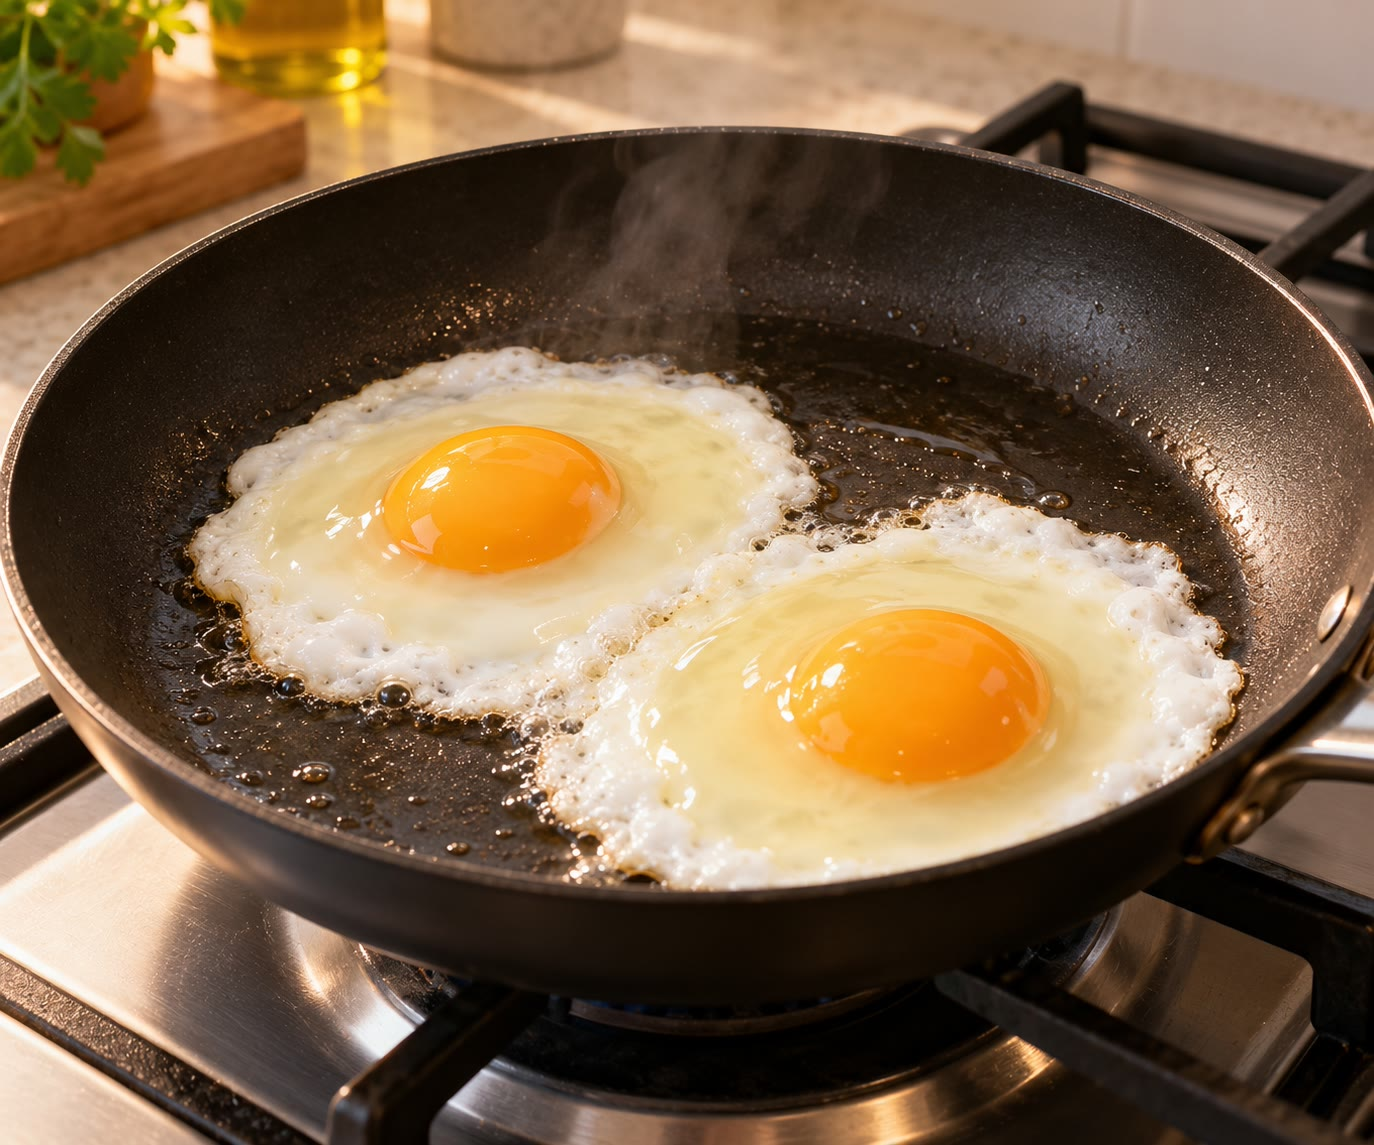
\includegraphics[width=0.5\linewidth]{images/book3/ai/b2-30-eggs.jpg}

{\small Eieren bakken. De eiwitten in het eiwit ontvouwen zich bij verhitten en binden aan elkaar: de
doorschijnende vloeistof wordt een ondoorzichtige witte vaste stof. Er breekt geen enkele \omterm{def:b2:biomolecules:peptide}{peptidebinding}; de verandering zit in de manier waarop
de ketens gevouwen zijn (illustratie).}
\end{omfigure}

\section{Koolhydraten}

\begin{definition}[D en L]\label{def:b2:biomolecules:d-l}
Een suiker of een aminozuur wordt in fischerprojectie getekend met zijn meest geoxideerde koolstofatoom bovenaan. Het is
D als de \ce{OH} op het stereocentrum dat het verst van de top ligt (of, voor een $\alpha$-aminozuur, de
\ce{NH2} op het $\alpha$-koolstofatoom) naar rechts wijst, en L als hij naar links wijst. De descriptoren
vergelijken configuraties met die van glyceraldehyde; het zijn niet de CIP-descriptoren.
\end{definition}

\begin{definition}[Monosachariden]\label{def:b2:biomolecules:sugar}
Een \emph{monosacharide}\index{monosacharide} is een polyhydroxyaldehyde of -keton, meestal
\ce{C_nH_{2n}O_n} met $n$ van 3 tot 7, dat niet tot kleinere suikers gehydrolyseerd kan worden. Een
\emph{aldose}\index{aldose} heeft een aldehydegroep op C1, een \emph{ketose}\index{ketose} een ketongroep,
meestal op C2. Glucose is een aldohexose, fructose een ketohexose.
\end{definition}

In water is een aldohexose bijna volledig cyclisch: de \ce{OH} op C5 addeert aan het aldehyde en vormt een
zesledige hemiacetaalring (een pyranose). De cyclisatie creëert een nieuw stereocentrum op C1.

\begin{definition}[Anomeren]\label{def:b2:biomolecules:anomer}
In een \emph{haworthprojectie}\index{haworthprojectie} wordt de ring van een cyclische suiker plat getekend,
loodrecht op de pagina, met zijn zuurstofatoom achteraan rechts en zijn substituenten boven of onder de
ring. Het hemiacetaalkoolstofatoom (C1 van een \omterm{def:b2:biomolecules:sugar}{aldose}) is het \emph{anomere koolstofatoom}\index{anomeer koolstofatoom}; de
twee configuraties die het kan aannemen, geven twee diastereo-isomeren, de \emph{anomeren}\index{anomeren}: bij een D-suiker
heeft $\alpha$ de anomere \ce{OH} onder de ring (tegenover de \ce{CH2OH}), $\beta$ erboven. In
water gaan de anomeren via de open keten in elkaar over, en de optische rotatie van een pas opgelost
anomeer verschuift naar een evenwichtswaarde: \emph{mutarotatie}\index{mutarotatie}.
\end{definition}

\begin{omfigure}
\setchemfig{atom sep=1.7em}
\begin{minipage}[c]{0.24\linewidth}\centering
\chemfig{CHO-[6]C(-[4]H)(-[0]OH)-[6]C(-[4,,,2]HO)(-[0]H)-[6]C(-[4]H)(-[0]OH)-[6]C(-[4]H)(-[0]OH)-[6]CH_2OH}
\end{minipage}%
\begin{minipage}[c]{0.37\linewidth}\centering
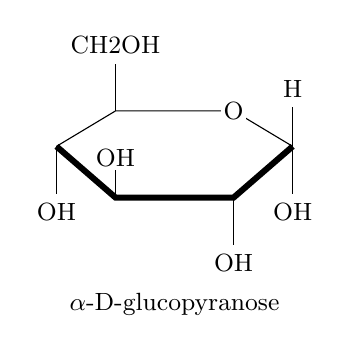
\begin{tikzpicture}[x=1cm, y=1cm, font=\small]
\coordinate (C4) at (-1.5,0); \coordinate (C3) at (-0.75,-0.65); \coordinate (C2) at (0.75,-0.65);
\coordinate (C1) at (1.5,0); \coordinate (O) at (0.75,0.45); \coordinate (C5) at (-0.75,0.45);
\draw (C5) -- (O) -- (C1); \draw (C4) -- (C5);
\draw[line width=2.2pt] (C4) -- (C3) -- (C2) -- (C1);
\node[fill=white, inner sep=1pt] at (O) {O};
\draw (C5) -- ++(0,0.6) node[above] {\ce{CH2OH}};
\draw (C1) -- ++(0,-0.6) node[below] {OH}; \draw (C1) -- ++(0,0.5) node[above] {H};
\draw (C2) -- ++(0,-0.6) node[below] {OH}; \draw (C3) -- ++(0,0.35) node[above, inner sep=1pt] {OH};
\draw (C4) -- ++(0,-0.6) node[below] {OH};
\node at (0,-2.0) {$\alpha$-D-glucopyranose};
\end{tikzpicture}
\end{minipage}%
\begin{minipage}[c]{0.37\linewidth}\centering
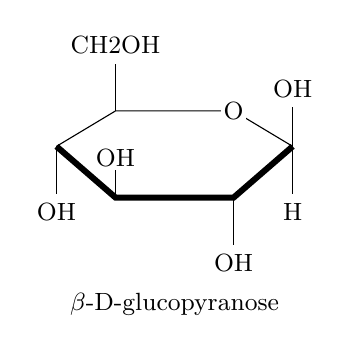
\begin{tikzpicture}[x=1cm, y=1cm, font=\small]
\coordinate (C4) at (-1.5,0); \coordinate (C3) at (-0.75,-0.65); \coordinate (C2) at (0.75,-0.65);
\coordinate (C1) at (1.5,0); \coordinate (O) at (0.75,0.45); \coordinate (C5) at (-0.75,0.45);
\draw (C5) -- (O) -- (C1); \draw (C4) -- (C5);
\draw[line width=2.2pt] (C4) -- (C3) -- (C2) -- (C1);
\node[fill=white, inner sep=1pt] at (O) {O};
\draw (C5) -- ++(0,0.6) node[above] {\ce{CH2OH}};
\draw (C1) -- ++(0,0.5) node[above] {OH}; \draw (C1) -- ++(0,-0.6) node[below] {H};
\draw (C2) -- ++(0,-0.6) node[below] {OH}; \draw (C3) -- ++(0,0.35) node[above, inner sep=1pt] {OH};
\draw (C4) -- ++(0,-0.6) node[below] {OH};
\node at (0,-2.0) {$\beta$-D-glucopyranose};
\end{tikzpicture}
\end{minipage}
\par\vspace{6pt}

{\small D-Glucose. Links: de open keten in fischerprojectie, \ce{OH} op C5 naar rechts (D). Midden
en rechts: de twee \omterm{def:b2:biomolecules:anomer}{pyranose-anomeren} in \omterm{def:b2:biomolecules:anomer}{haworthprojectie}; de groepen rechts in de
fischerprojectie wijzen omlaag, die links omhoog, en C5 draagt de \ce{CH2OH} omhoog. De \omterm{def:b2:biomolecules:anomer}{anomeren}
verschillen alleen op C1. De waterstofatomen op C2 tot C5 zijn weggelaten.}
\end{omfigure}

\begin{method}[Van Fischer naar Haworth (D-aldopyranose)]\label{met:b2:biomolecules:haworth}
\begin{enumerate}
  \item Teken de ring met O achteraan rechts, C1 rechts, dan C2, C3, C4 met de klok mee langs de
        voorkant en links, C5 achteraan links.
  \item Groepen rechts in de fischerprojectie gaan omlaag, groepen links gaan omhoog.
  \item Op C5 (D-reeks) gaat de \ce{CH2OH} omhoog.
  \item Op C1 gaat de \ce{OH} omlaag voor $\alpha$, omhoog voor $\beta$.
\end{enumerate}
\end{method}

\begin{proposition}[Mutarotatie-evenwicht]\label{prop:b2:biomolecules:mutarotation}
Als de specifieke rotaties van de zuivere \omterm{def:b2:biomolecules:anomer}{anomeren} $[\alpha]_\alpha$ en $[\alpha]_\beta$ zijn en die van het
evenwichtsmengsel $[\alpha]_{\mathrm{eq}}$, dan is de molfractie van het $\alpha$-anomeer bij
evenwicht
\begin{equation*}
x_\alpha = \frac{[\alpha]_{\mathrm{eq}} - [\alpha]_\beta}{[\alpha]_\alpha - [\alpha]_\beta}.
\end{equation*}
\end{proposition}

\begin{proof}
De open keten is een heel kleine fractie van het mengsel en wordt verwaarloosd. De rotaties van de twee \omterm{def:b2:biomolecules:anomer}{anomeren}
tellen op naar verhouding van hun concentraties (wet van Biot, deel van jaar~1); omdat ze dezelfde molaire
massa hebben, is $[\alpha]_{\mathrm{eq}} = x_\alpha[\alpha]_\alpha + (1 - x_\alpha)[\alpha]_\beta$, wat opgelost wordt
naar $x_\alpha$.
\end{proof}

D-Glucose heeft bij evenwicht in water $[\alpha] = +52.7$ (in \unit{\degree\,dm^{-1}\,g^{-1}\,mL}).
Met anomeerrotaties van $+112$ en $+18.7$ (gegevens voor de oefening) is $x_\alpha = (52.7 - 18.7)/(112 - 18.7)
\approx 0.36$: ongeveer 36~\% $\alpha$ en 64~\% $\beta$. Het $\beta$-anomeer, met al zijn
substituenten equatoriaal in de stoel, is het stabielste.
% ledger: rot:glucose-eq

\begin{definition}[Glycosiden]\label{def:b2:biomolecules:glycoside}
Een \emph{glycoside}\index{glycoside} is het acetaal dat ontstaat wanneer de anomere \ce{OH} van een suiker vervangen wordt
door een groep \ce{OR} van een alcohol, vaak een andere suiker; de binding van het \omterm{def:b2:biomolecules:anomer}{anomere koolstofatoom} naar dat
zuurstofatoom is de \emph{glycosidische binding}\index{glycosidische binding}. Een \emph{reducerende suiker}\index{reducerende suiker}
is een suiker die milde oxidatoren zoals de oplossing van Fehling of het reagens van Tollens reduceert.
\end{definition}

\begin{proposition}[Reducerend of niet]\label{prop:b2:biomolecules:reducing}
Een suiker met een vrije hemiacetaal- (of hemiketaal)groep is reducerend; een \omterm{def:b2:biomolecules:glycoside}{glycoside} waarvan de \omterm{def:b2:biomolecules:anomer}{anomere koolstofatomen}
allemaal in \omterm{def:b2:biomolecules:glycoside}{glycosidische bindingen} betrokken zijn, is dat niet.
\end{proposition}

\begin{proof}[Redenering]
Een hemiacetaal staat in evenwicht met de open keten, waarvan de aldehydegroep door het reagens geoxideerd wordt;
het evenwicht opent dan meer ringen tot alle suiker gereageerd heeft. Een acetaal gaat in neutraal of
basisch water niet open: het \omterm{def:b2:biomolecules:anomer}{anomere koolstofatoom} blijft vergrendeld, zonder aldehyde om te oxideren.
\end{proof}

Maltose (twee glucosen, C1 van de ene gebonden aan O4 van de andere) houdt één vrij hemiacetaal en is reducerend;
sacharose verbindt de \omterm{def:b2:biomolecules:anomer}{anomere koolstofatomen} van glucose en fructose met elkaar en is dat niet. Zetmeel en
cellulose zijn allebei ketens van glucose, verbonden C1--O4: $\alpha$ in zetmeel, dat zich oprolt en verteerd wordt;
$\beta$ in cellulose, waarvan de rechte ketens zich tot vezels schikken die door waterstofbruggen bijeengehouden worden.

\section{Lipiden}

\begin{definition}[Lipiden]\label{def:b2:biomolecules:lipid}
Een \emph{vetzuur}\index{vetzuur} is een carbonzuur met een lange onvertakte keten, meestal van 12 tot
22 koolstofatomen, verzadigd of met (\textit{Z})-dubbele bindingen. Een \emph{triglyceride}\index{triglyceride} is de
triester van propaan-1,2,3-triol (glycerol) met drie vetzuren. Een
\emph{fosfolipide}\index{fosfolipide} is een diester van glycerol met twee vetzuren waarvan de derde
positie een fosfaatgroep draagt die aan een kleine polaire groep gebonden is.
\end{definition}

De (\textit{Z})-dubbele bindingen buigen de ketens, die zich dan slecht stapelen: stearinezuur (18 koolstofatomen,
verzadigd) smelt bij \qty{69}{\degreeCelsius}, oliezuur (18 koolstofatomen, één \textit{Z}-dubbele binding) bij
\qty{13}{\degreeCelsius}. Vetten die rijk zijn aan verzadigde ketens zijn vast bij kamertemperatuur; oliën, rijk aan
onverzadigde ketens, zijn vloeibaar. \omterm{def:b2:biomolecules:lipid}{Triglyceriden} worden verzeept tot glycerol en zepen
(\cref{ch:b2:acyl-substitution}).
% ledger: mp:stearic, mp:oleic

\begin{omfigure}
\begin{tikzpicture}[x=1cm, y=1cm]
\foreach \i in {0,1,2,3,4,5,6,7,8,9}{
  \fill[omDef!60] (0.6*\i,1.6) circle (0.17);
  \draw[thick, black!70] (0.6*\i-0.06,1.43) .. controls (0.6*\i-0.12,1.2) and (0.6*\i,1.0) .. (0.6*\i-0.06,0.75);
  \draw[thick, black!70] (0.6*\i+0.06,1.43) .. controls (0.6*\i+0.12,1.2) and (0.6*\i,1.0) .. (0.6*\i+0.06,0.75);
  \fill[omDef!60] (0.6*\i,-0.6) circle (0.17);
  \draw[thick, black!70] (0.6*\i-0.06,-0.43) .. controls (0.6*\i-0.12,-0.2) and (0.6*\i,0.0) .. (0.6*\i-0.06,0.25);
  \draw[thick, black!70] (0.6*\i+0.06,-0.43) .. controls (0.6*\i+0.12,-0.2) and (0.6*\i,0.0) .. (0.6*\i+0.06,0.25);
}
\node[font=\small, anchor=west] at (6.0,2.2) {water};
\node[font=\small, anchor=west] at (6.0,0.5) {koolwaterstofkern};
\node[font=\small, anchor=west] at (6.0,-1.2) {water};
\draw[densely dotted] (5.6,1.6) -- (6.0,1.6) node[right, font=\footnotesize] {polaire koppen};
\draw[densely dotted] (5.6,1.05) -- (6.0,1.05) node[right, font=\footnotesize] {twee vetzuurstaarten};
\end{tikzpicture}
\par\vspace{4pt}

{\small Een fosfolipidedubbellaag, schematisch: de polaire koppen zijn aan beide kanten naar het water gericht, de
koolwaterstofstaarten ontmoeten elkaar binnenin. Celmembranen zijn op deze structuur gebouwd; zepen, met één staart per
kop, vormen in plaats daarvan kleine bolletjes met de staarten binnenin, micellen genoemd.}
\end{omfigure}

\section{Nucleotiden}

\begin{definition}[Nucleotiden]\label{def:b2:biomolecules:nucleotide}
Een \emph{nucleobase}\index{nucleobase} is een stikstofheterocyclus: adenine (A) en guanine (G), purinen;
cytosine (C), thymine (T) en uracil (U), pyrimidinen. Een \emph{nucleoside}\index{nucleoside} is een
nucleobase die via een stikstofatoom gebonden is aan C1 van ribose of 2-desoxyribose (een $N$-glycoside). Een
\emph{nucleotide}\index{nucleotide} is een fosfaatester van een nucleoside. In nucleïnezuren zijn de
nucleotiden verbonden door \emph{fosfodiësterbindingen}\index{fosfodiesterbinding@fosfodiësterbinding}: één fosfaat verbindt
O3 van de ene suiker met O5 van de volgende.
\end{definition}

DNA gebruikt 2-desoxyribose en de basen A, G, C, T; RNA gebruikt ribose en U in plaats van T. De keten heeft een
richting, van haar 5$'$-uiteinde naar haar 3$'$-uiteinde, en de fosfaten, geïoniseerd bij fysiologische pH, maken er een
polyanion van. Twee DNA-strengen lopen in tegengestelde richting en worden bijeengehouden door waterstofbruggen tussen
basen die tegenover elkaar staan.

\begin{proposition}[Basenparing]\label{prop:b2:biomolecules:pairing}
In dubbelstrengs DNA paart adenine met thymine via twee waterstofbruggen, en guanine met cytosine
via drie.
\end{proposition}

\begin{proof}[Redenering]
De paren zijn die waarvan de randen donoren (\ce{N-H}) tegenover acceptoren (zuurstof van \ce{C=O},
ringstikstof) plaatsen op de juiste afstanden, met een purine tegenover een pyrimidine, zodat elk paar dezelfde
breedte heeft. A biedt \ce{N-H} (zijn aminogroep) en een ring-\ce{N}; T biedt \ce{C=O} en \ce{N-H}: twee bruggen. G
biedt \ce{C=O}, \ce{N-H} en \ce{N-H} (amino); C biedt \ce{N-H} (amino), \ce{N} en \ce{C=O}: drie
bruggen. De figuur toont ze.
\end{proof}

\begin{omfigure}
\setchemfig{atom sep=1.7em}
\chemfig{?[a](-[:90]CH_3)-[:-30](=[:30]@{to}O)-[:-90]N(-[:-30]@{th}H)-[:-150](=[:-90]O)-[:150]N(-[:-150]R)-[:90]?[a,2]}%
\hspace{2.3em}%
\raisebox{-1.0em}{\chemfig{?[a](-[:150]N(-[:90]H)-[:210]@{ah}H)-[:30]?[b](-[:78]N=[:6]-[:-66]N(-[:-30]R)-[:-138]?[c])=[:-30]?[c]-[:-90]N=[:-150]-[:150]@{an}N?[a,2]}}
\chemmove{\draw[-, densely dotted, thick](to)--(ah); \draw[-, densely dotted, thick](th)--(an);}
\hspace{1.5em}
\chemfig{?[a]-[:-30](-[:30]N(-[:90]H)-[:-30]@{ch}H)=[:-90]@{cn}N-[:-150](=[:-90]@{co}O)-[:150]N(-[:-150]R)-[:90]?[a,2]}%
\hspace{2.3em}%
\raisebox{-0.6em}{\chemfig{?[a](=[:150]@{go}O)-[:30]?[b](-[:78]N=[:6]-[:-66]N(-[:-30]R)-[:-138]?[c])=[:-30]?[c]-[:-90]N=[:-150](-[:-90]N(-[:-30]H)-[:-150]@{gh}H)-[:150]N?[a](-[:180]@{gn}H)}}
\chemmove{\draw[-, densely dotted, thick](ch)--(go); \draw[-, densely dotted, thick](cn)--(gn);
  \draw[-, densely dotted, thick](co)--(gh);}
\par\vspace{6pt}

{\small De twee basenparen van DNA. Links: thymine en adenine, twee waterstofbruggen (gestippeld). Rechts:
cytosine en guanine, drie. R is de desoxyribose van elke streng; de twee groepen R van een paar wijzen naar
dezelfde kant, naar de twee ruggengraten.}
\end{omfigure}

\begin{history}[De suikers, 1891]
\begin{minipage}[t]{0.18\linewidth}
\vspace{0pt}
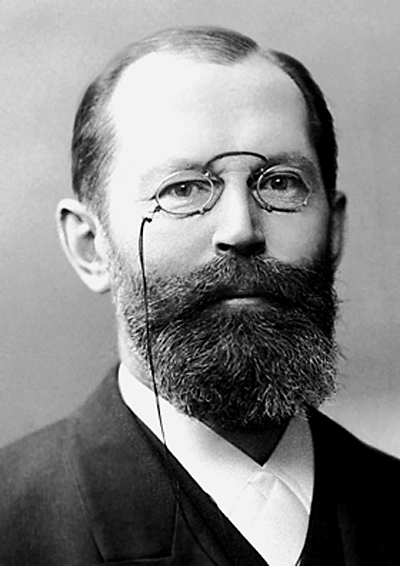
\includegraphics[width=\linewidth]{images/book3/fischer.jpg}
\end{minipage}\hfill
\begin{minipage}[t]{0.78\linewidth}
\vspace{0pt}
Emil Fischer bepaalde tegen 1891 de configuraties van glucose en van zijn isomeren, nog voor enige
fysische methode een molecuul kon zien: door suikers in elkaar om te zetten en de verkregen
stereo-isomeren te tellen. De projectie die hij uitvond om ze op te schrijven, draagt nog altijd zijn naam. Hij maakte ook
de eerste synthetische \omterm{def:b2:biomolecules:peptide}{peptiden}, en kreeg in 1902 de Nobelprijs voor de Scheikunde. (Portret: Atelier
Victoria, Berlijn, rond 1895, publiek domein; Wikimedia Commons.)
\end{minipage}
\end{history}

\section{Oefeningen}

\begin{exercise}[$\star$]\label{exo:b2:biomolecules:1}
Teken alanine als \omterm{def:b2:biomolecules:amino-acid}{zwitterion}, en daarna de vormen die overheersen bij pH 1 en bij pH 12.
\end{exercise}

\begin{exercise}[$\star$]\label{exo:b2:biomolecules:2}
Bereken het \omterm{def:b2:biomolecules:amino-acid}{iso-elektrisch punt} van glycine, en dat van alanine ($\mathrm pK_a$ 2.35 en 9.87).
\end{exercise}

\begin{exercise}[$\star$]\label{exo:b2:biomolecules:3}
Teken het dipeptide Ala--Gly en omcirkel zijn \omterm{def:b2:biomolecules:peptide}{peptidebinding}. Waarin verschilt het van Gly--Ala?
\end{exercise}

\begin{exercise}[$\star$]\label{exo:b2:biomolecules:4}
In een fischerprojectie met \ce{COOH} bovenaan en de \omterm{def:b2:biomolecules:amino-acid}{zijketen} \ce{CH2OH} onderaan wijst de
\ce{NH2} van serine naar links. Is het D of L? Geef zijn CIP-descriptor.
\end{exercise}

\begin{exercise}[$\star\star$]\label{exo:b2:biomolecules:5}
Geef de nettolading van het tripeptide Lys--Gly--Asp bij pH 1, 7 en 12.
\end{exercise}

\begin{exercise}[$\star\star$]\label{exo:b2:biomolecules:6}
Waarom gebruikt men een \omterm{def:b2:biomolecules:peptide}{koppelingsreagens} om een \omterm{def:b2:biomolecules:peptide}{peptidebinding} te maken, eerder dan een \omterm{def:b2:acyl-substitution:derivative}{acylchloride} van het beschermde
aminozuur, gemaakt met thionylchloride, en verhitting?
\end{exercise}

\begin{exercise}[$\star\star$]\label{exo:b2:biomolecules:7}
D-Fructose cycliseert via zijn \ce{OH} op C5 met het keton op C2. Geef de grootte van de ring en teken
$\beta$-D-fructofuranose in \omterm{def:b2:biomolecules:anomer}{haworthprojectie}.
\end{exercise}

\begin{exercise}[$\star\star$]\label{exo:b2:biomolecules:8}
De zuivere \omterm{def:b2:biomolecules:anomer}{anomeren} van D-galactose hebben specifieke rotaties van $+150.7$ ($\alpha$) en $+52.8$ ($\beta$), en
het evenwichtsmengsel $+80.2$ (gegevens voor de oefening). Bereken de evenwichtssamenstelling.
\end{exercise}

\begin{exercise}[$\star\star$]\label{exo:b2:biomolecules:9}
Leg uit waarom maltose de oplossing van Fehling reduceert en sacharose niet, en waarom sacharose dat wel doet na
verhitten met verdund zuur.
\end{exercise}

\begin{exercise}[$\star\star\star$]\label{exo:b2:biomolecules:10}
Het verzepingsgetal van een vet is de massa kaliumhydroxide, in mg, die 1~g ervan verzeept.
Bereken het voor trioleïne, \ce{C57H104O6}, en leg uit waarom een vet met kortere ketens een hogere waarde heeft.
\end{exercise}

\begin{exercise}[$\star\star\star$]\label{exo:b2:biomolecules:11}
Plan de synthese van Gly--Ala uit glycine en alanine: beschermende groepen, activering, koppeling,
ontscherming, met een orthogonaal paar.
\end{exercise}

\begin{exercise}[$\star\star\star$]\label{exo:b2:biomolecules:12}
Schrijf de streng op die complementair is aan 5$'$-ATGCGT-3$'$, vanaf haar 5$'$-uiteinde, en tel de waterstofbruggen
die de dubbele streng bijeenhouden.
\end{exercise}

\section{Probleem: aspartaam}

\begin{problem}[{Weekendprobleem --- de twee aminozuren en hun configuraties, de lading van het
dipeptide tegen de pH, zijn synthese en het $\alpha$/$\beta$-probleem, en zijn hydrolyse in een
frisdrank}]
\label{pb:b2:biomolecules:1}
Aspartaam is de methylester van het dipeptide dat gevormd wordt door de $\alpha$-carbonzuurgroep van L-asparaginezuur
met de aminogroep van L-fenylalanine. Gegevens: $\mathrm pK_a$ van asparaginezuur 2.0, 3.9 en 9.9 (modelwaarden
voor de groepen van het dipeptide). Molaire massa's (\unit{g/mol}): C 12.011, H 1.008, N 14.007,
O 15.999.
% ledger: use:aspartame, pka:asp1, pka:asp2, pka:asp3, aw:C, aw:H, aw:N, aw:O

\medskip
\noindent\textbf{Deel I --- De twee aminozuren.}
\begin{enumerate}
  \item Geef de drie verbindingen die vrijkomen bij de volledige hydrolyse van aspartaam.
  \item Teken L-asparaginezuur en L-fenylalanine in fischerprojectie.
  \item Geef de CIP-descriptor van elk stereocentrum.
  \item Hoeveel stereo-isomeren heeft aspartaam?
  \item Teken aspartaam en markeer de \omterm{def:b2:biomolecules:peptide}{peptidebinding} en de ester.
  \item Waarom is de configuratie van elk aminozuur belangrijk voor de zoete smaak?
\end{enumerate}

\medskip
\noindent\textbf{Deel II --- Lading tegen de pH.}
\begin{enumerate}[resume]
  \item Som de ioniseerbare groepen van aspartaam op. Waarom hoort de C-terminus daar niet bij?
  \item Geef met de modelwaarden de nettolading bij pH 2.
  \item Hetzelfde bij pH 7.
  \item Hetzelfde bij pH 12.
  \item Schat het \omterm{def:b2:biomolecules:amino-acid}{iso-elektrisch punt} in dit model.
  \item Waarom zouden de echte $\mathrm pK_a$-waarden van het dipeptide verschillen van die van vrij
        asparaginezuur?
\end{enumerate}

\medskip
\noindent\textbf{Deel III --- Synthese.}
\begin{enumerate}[resume]
  \item Waarom kun je asparaginezuur en de methylester van fenylalanine niet gewoon samen verhitten?
  \item Welke groepen van asparaginezuur moeten beschermd worden?
  \item Wat doet een \omterm{def:b2:biomolecules:peptide}{koppelingsreagens} met de vrije carbonzuurgroep?
  \item Asparaginezuur heeft twee carbonzuurgroepen. Wat ontstaat er als de verkeerde gekoppeld wordt?
  \item Stel een orthogonale bescherming voor die alleen de $\alpha$-carbonzuurgroep vrij laat, en de
        verwijdering ervan.
  \item Waarom mag het geactiveerde aminozuur niet te lang onder basische omstandigheden blijven?
  \item Schrijf de volgorde van de stappen op.
\end{enumerate}

\medskip
\noindent\textbf{Deel IV --- Hydrolyse in een frisdrank.}
\begin{enumerate}[resume]
  \item Welke bindingen van aspartaam kunnen in een zure drank gehydrolyseerd worden? Welke eerst?
  \item Geef de producten van de hydrolyse van alleen de ester.
  \item Waarom smaakt een oude drank minder zoet?
  \item Bereken de molaire massa van aspartaam, \ce{C14H18N2O5}.
  \item Bereken de hoeveelheid aspartaam in een blikje dat \qty{180}{mg} bevat.
  \item Geef de massa methanol die vrijkomt bij de volledige hydrolyse van \qty{180}{mg}
        aspartaam.
\end{enumerate}
\end{problem}
